\subsubsection{Funktionsweise}

Bei der Bilderzeugung, ausgehend von Szenen, welche viel Geometrie beinhalten bzw. bei Szenen 
die generelle BRDF's verwenden eignet sich der \nameref{ch:Content1:sec:Path Tracer}.
Der \nameref{ch:Content1:sec:Path Tracer} ist in Hinsicht der Beleuchtung komplett. Deshalb lässt sich damit
\textit{Global Illumination} erreichen. Der hier verwendete \nameref{ch:Content1:sec:Path Tracer} in 
\cite{Benty18} verwendet eine klassische Umsetzung.\par
Der Path Tracer beruht auf Erkenntnisse der Lösung der allgemeinen Rendergleichung.\nameref{eq:Allgemeine Rendergleichung}

\begin{equation}\label{eq:Allgemeine Rendergleichung}
    I(x,{x}^{'}) = g(x,{x}^{'}) * \biggl[\epsilon(x,{x}^{'}) + 
    \int_{S}^{} \rho(x,{x}^{'},{x}^{''})
    I({x}^{'},{x}^{''}d{x}^{''})\biggr] 
\end{equation}

Sie beschreibt den Energietransport \textit{I} von einem Punkt ${x}^{'}$
zu einem Punkt x. Dabei ist ein maßgebender Faktor der Geometrieterm \textit{g},
der die relative Lage der beiden Punkte zueinander im Raum beschreibt.
Ein weiterer Faktor ist die Abstrahlung \textit{$\epsilon$} von ${x}^{'}$ nach x. 
Beeinflusst wird der Energiefluss auch durch
die bidirektionale Verteilungsfunktion \textit{$\rho$}, welche Aufschluss über
das einfallende Licht von einem Punkt ${x}^{''}$ über ${x}^{'}$ zu x gibt.\par
Die Schlussfolgerung aus dieser Gleichung \nameref{eq:Allgemeine Rendergleichung} ist: Die transportierte
Intensität von einem Licht zu einem Anderen ist die Summe des ausgestrahlten Lichts 
und das ausgestrahlte Licht zu x von allen anderen Oberflächen.

Ausgehend von der Rendergleichung \nameref{eq:Allgemeine Rendergleichung} lässt sich
die vollständige Transportgleichung\nameref{eq:vollständige Transportgleichung} des \nameref{ch:Content1:sec:Path Tracer}
beschreiben.
Wie von \cite{marschner2009fundamentals} beschrieben wird ausgehend von der vollständigen Transportgleichung
\nameref{eq:vollständige Transportgleichung}

\begin{equation}\label{eq:vollständige Transportgleichung}
    L_s(k_0) = L_e(k_0) + \int_{all(k_i)}^{} \rho(k_i, k_0)*L_f(k_i)*cos(\theta_i)d\theta_i
\end{equation}

der vollständige Lichttransport beschrieben. Man kann deutlich die Ähnlichkeit
zu \nameref{eq:Allgemeine Rendergleichung} erkennen. Wir haben den Emissionsterm, die relative Lage der 
Punkte zueinander und die bidirektionale Verteilungsfunktion welche den Energietransport
beeinflussen.

\begin{figure}[H]
    \centering
    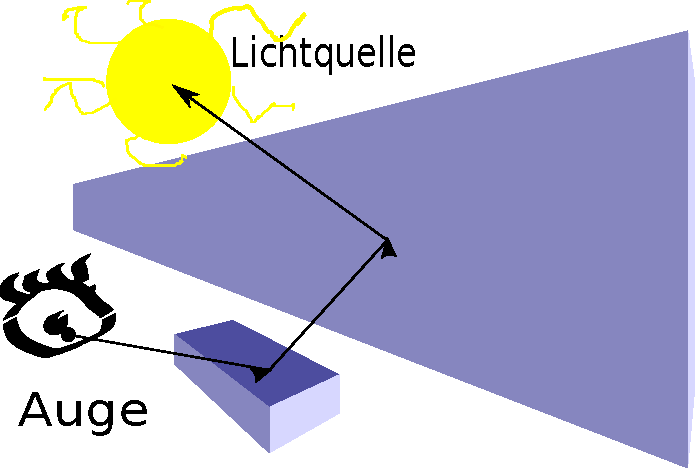
\includegraphics[width=0.7\linewidth]{content/PathTracer/Bilder/Grundkonzept_path_tracing.pdf}
    \label{pic::Grundkonzept Path Tracing}
    \caption{Grundkonzept path tracer}
\end{figure}

\subsubsection{Monte-Carlo-Integration}
Mit der Monte Carlo Integration approximieren wir die Rendergleichung.\par 
Bei gegebener Dimensionalität n des Renderintegrals und der 
Wahrscheinlichkeitsdichtefunktion $\rho(x_i)$
\cite{KK02}

\begin{equation}\label{eq:Monte-Carlo}
    E\biggl[\frac{1}{k}\sum_{i=1}^{k}\frac{f(X_{i}}{\rho(X_{i})})\biggl] = \int_{[0,1]^{n}}f(x)dx
\end{equation}

Dabei wird das n-dimensionale Integral\nameref{eq:vollständige Transportgleichung} approximiert. Die Dichtefunktion $\rho(x_i)$ 
beschreibt deutet an, dass hierbei die Stichproben auch nicht-uniform 
genommen werden können. Varianzreduktionsmethoden machen sich diese Dichtefunktion zu Nutze um 
ein besseres Ergebnis zu bekommen.
\cite{caflisch_1998}
Konvergenzrate, unabhängig von der Dimension unseres Tracers.\textit{O}($N^{-\frac{1}{2}}$).
Sie ist robust, das heißt Exaktheit hängt nur vom ungenauesten Parameter ab. Eine Variante des Verfahrens, 
Monte Carlo Quadratur, wird mit quasi zufälligen Sequenzen \nameref{ch:Content1:sec:Quasi-Zufallsfolgen}, 
welche eine niedrige Abweichung aufweisen, durchgeführt. Laufzeit quasi-Monte Carlo \textit{O}(($\log N)^{k}N^{-1}$).
Um die Konvergenzrate zu steigern liegen eine Reihe von Varianzreduktionsmethoden vor.

Abseits dieser herkömmlichen Strategien zeigen wir hier die Steigerung der 
visuellen Qualität durch blue noise Fehlerverteilung im Bildraum.

\begin{equation}\label{eq:Monte-Carlo-Varianz}
    V[X] = E\biggl[(X-E[X])^{2}\biggl] = E[X^{2}]
    - E[X]^{2}
\end{equation}

Die Varianz \nameref{eq:Monte-Carlo-Varianz} ist ein quadratischer Fehler.

\subsubsection{DirectX Raytracing}

\begin{figure}[H]
    \centering
    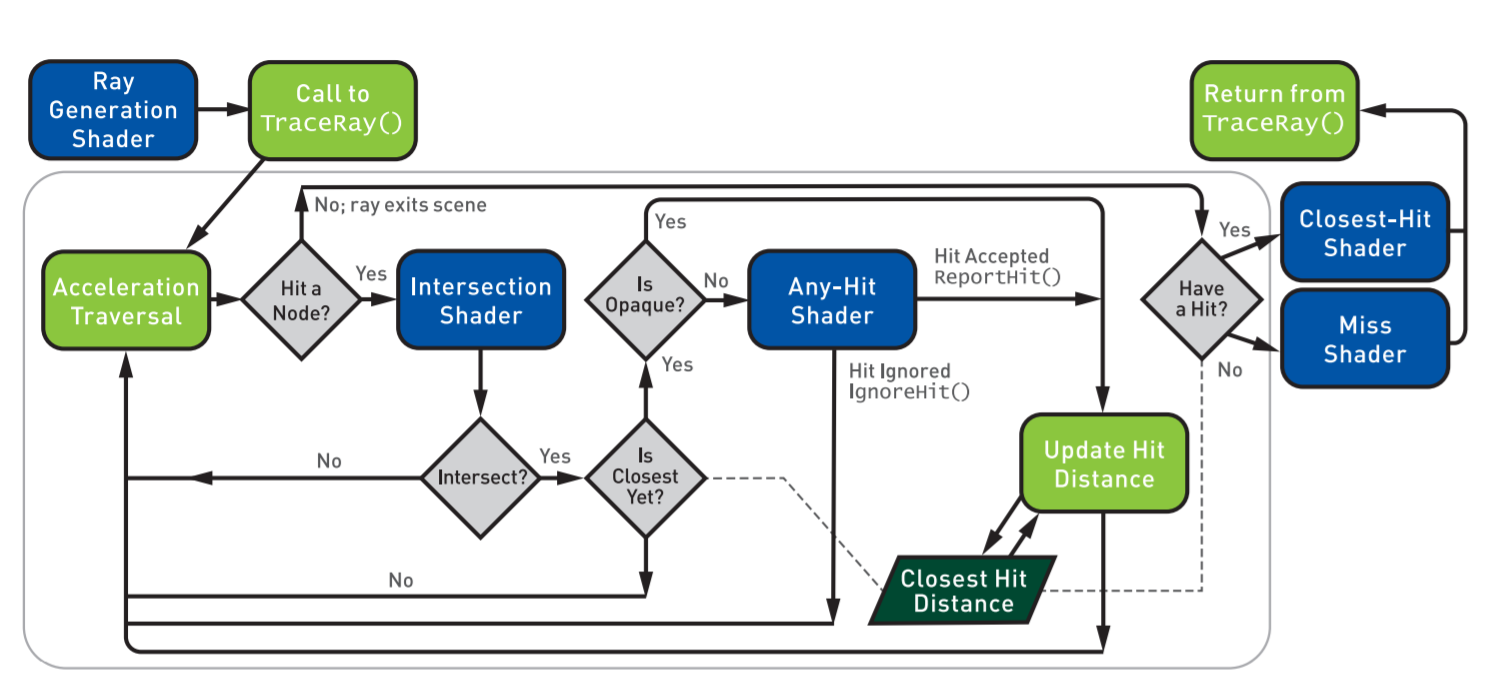
\includegraphics[width=\linewidth]{content/PathTracer/Bilder/DirectXRaytracingPipeline.png}
    \caption{DirectX Raytracing Pipeline aus \cite{Haines2019}}
    \label{pic:DirectXRaytracingPipeline}
\end{figure}

In \ref{pic:DirectXRaytracingPipeline} lässt sich der Beginn (Generierung eines Strahles) der neuen Pipeline
durch den programmierbaren \textbf{Ray Generation shader} erkennen.

\begin{algorithm}[H]
    \caption{Beispielhafter minimalistischer Ray Generation Shader}
    \begin{algorithmic}[1]
        \State [shader(\dq raygeneration \dq)]
        \State launchIndex = DispatchRaysIndex().xy;
        \For{(int i = 0; i < numberOfRays;i++)}
            \State float shadowRayMult = TraceRay(gRtScene,
            RAY\_FLAG\_ACCEPT\_FIRST\_HIT \_AND\_END\_SEARCH |
            RAY\_FLAG\_SKIP\_CLOSEST\_HIT\_SHADER,
            0xFF, 0, hitProgramCount, 0, ray, payload);
            \State float indirectRayColor = TraceRay(gRtScene, 0, 0xFF, 1, hitProgramCount, 1, rayColor, payload);
            \State color = shadowRayMult * shadingColor + computeindirectLighting(indirectRayColor);
        \EndFor
        \State output[id] = color;
    \end{algorithmic}
    \label{alg:Ray Gen}
\end{algorithm}

Mit Hilfe der Methode \textbf{TraceRay()} werden dann zur Beleuchtungsberechnung 
die Strahlen verschossen. Damit diese Methode richtig arbeiten kann übergeben wir neben unseren Strahl 
unter Anderem  unsere Szene inklusive Beschleunigungsstruktur, rayflags 
(beeinflussen Transparaenz, Culling, Abbruch)\cite{RayFlags} und einen payload.
Mit dem \textit{$payload_t$} Typ können wir einen struct mit Informationen jedem einzelnen Strahl mitgeben.

\begin{algorithm}[H]
    \caption{beispielhafter payload}
    \begin{algorithmic}[1]
        \State struct RayPayload = {
            \State        float4 color, uint32 seed, uint32 depth
            \State };
        \end{algorithmic}
        \label{alg:payload}
    \end{algorithm}
    
Diese Methode \textbf{TraceRay()} kann auch innerhalb der anderen Shader zum weiteren verschießen
von Strahlen verwendet werden. Beispiel beim Verschiessen vom Schattenstrahl: Flags 
RAY\_FLAG\_ACCEPT\_FIRST\_HIT\_AND\_END\_SEARCH, \newline
RAY\_FLAG\_SKIP\_CLOSEST\_HIT\_SHADER setzen, um unnötige 
Shadingberechnungen und weitere Schnittpunktberechnungen zu umgehen und mit einem Bit als payload 
die Sichtbarkeit zur Lichtquelle mitgeben.


Mit diesem beispielhaften payload können wir die Farbe akkumulieren, unseren verwendeten 
seed verwenden um z.B eine weiteren Strahlenschuss in einem Any-Hit Shader zu verwirklichen,  
solange die mit übergebene Rekursionstiefe in unserem payload eingehalten wird.  

\textbf{Intersection shader} führt die Schnittberechnungen durch.
Haben wir eine Szene, welche aus ausschließlich Dreiecken besteht, können wir
die auf Hardware standardmäßig gelieferte Implementierung übernehmen. 
Optionale Berechnungen für andere Geometrie können hier implementiert werden.
Bei einem gefundenen nähsten Schnittpunkt einer durchsichtigen Oberfläche wird der 
\textit{Any-hit shader} aufgerufen.
\textbf{Any-hit shaders} erlauben klassische \textit{Discards} oder informieren
über einen korrekten Schnitt. So können wir z.B. einen Alpha Test durchführen.

\begin{algorithm}[H]
    \caption{Any-Hit shader}
    \begin{algorithmic}[1]
        \State [shader(\dq anyhit \dq)]
        \If{(!alphaTest)} 
        \State IgnoreHit();
        \EndIf
    \end{algorithmic}
    \label{alg:any hit}
\end{algorithm}

Der \textbf{Closest-hit shader} berechnet den Schnittpunkt des Strahls mit der Geometrie
der Szene, die dem Strahlursprung am nähesten ist.
Mit der Kennzeichnung [shader(\dq closesthit \dq)] wird die Hauptmethode zur 
dessen Ausführung markiert. An dieser Stelle bietet es sich an die Shading Farbe 
mit der Schnittpunktinformation zu aktualisieren und/oder um eine Rekursionstiefe weiter 
zu gehen einen weiteren Strahl zu verschießen. 
Der \textbf{miss shader} wird immer dann ausgeführt, wenn ein Strahl die
Szenengeometrie nicht schneidet. Kann also für das Nachschauen in einer 
Environment Map verwendet werden. Im Folgenden \nameref{alg:Path Tracer Konzept}
nochmal vereinfacht in Pseudocode dargestellt, wobei die entsprechenden shader
im jeweiligen Codeabschnitt markiert sind.

\begin{algorithm}[H]
    \caption{Path Tracing Algorithmus}
    \begin{algorithmic}[1]
        \Procedure{Trace Path}{$BVH$}\Comment{verfolge Pfad durch Szene}
        \For{(x,y) $\in$ frame}
        \State strahl = verschiesseStrahlInPixel(x,y); // \textbf{ray generation shader}
        \For{blatt = bekommeBVHBlatt()}
        \State schnittpunkt = schneideGeometrie(strahl, blatt); //\textbf{Intersection shader}
        \If{schnittpunkt $\leq$ nähesterSchnittpunkt}
        \State aktualisiereNähestenSchnittpunkt();
        \EndIf
        \EndFor
        \If{Schnittpunkt gefunden}
        \State frame(x,y) = gebeFarbe(strahl,nähesterSchnittpunkt); //\textbf{closest-hit shader}
        \Else
        \State frame(x,y) = Umgebungskarte(x,y);//\textbf{miss shader}
        \EndIf
        \EndFor
        \EndProcedure
    \end{algorithmic}
    \label{alg:Path Tracer Konzept}
\end{algorithm}

\subsection{RenderGraph}
\todo{Give short introduction in the used rndergraph with its steps}




